\section{Methods}\label{sec:method}
The goal is to adapt a pretrained VLA to complete language-conditioned manipulation tasks on a target robot without collecting human demonstrations on that robot. We study multi-stage pick-and-place tasks: an instruction such as \emph{put the apple on the plate} requires approach, grasp, lift, transport, and release. The policy receives camera images, proprioception, and an instruction, predicts an action chunk, and executes a prefix before observing again. We evaluate complete-task success independently of the reward used for training.

\textbf{Target embodiment.} The CDPR suspends its end effector from four cables. Each cable runs from a fixed anchor to a position-controlled slider. The tool adds a yaw joint and a two-finger gripper. Each executed action is a normalized five-dimensional increment: Cartesian translation (up to 1.5\,cm per axis), yaw (up to 0.08\,rad), and gripper opening. A fixed inverse-kinematics controller converts the end-effector target to cable lengths. The policy therefore learns the mapping from images and language to Cartesian increments, while cable actuation remains hand-built. Observations are an overview and a wrist camera together with six proprioceptive values. SmolVLA was pretrained on 481 community datasets, which its authors describe as collected from a single robot type, the SO100 serial arm~\cite{smolvla}. A cable-driven parallel mechanism and this action interface are absent from that documented robotic data. We make no claim about images in its vision-language pretraining.

\textbf{Data contract.} We distinguish human demonstrations on the target robot (none are used), automatically generated trajectories used as supervised action targets, and assistance used only to choose starting states. Pretrained robot data enter only through the SmolVLA weights. Section~\ref{sec:lineage} reports each category for every ancestor of the evaluated controller.

Skills are acquired with their own instructions, success conditions, and starting states, whereas composition and evaluation start with an empty gripper and one complete-task instruction.


\subsection{Dense Acquisition, Binary Refinement, and Self-Imitation}\label{sec:skill_acquisition}
We use dense rewards only at the beginning of adaptation to learn a base policy for simple skills. Each skill has a distinct instruction and reset distribution:
\begin{itemize}
\item \textbf{Approach:} \emph{move to \textless object\textgreater}. Reach the named object with an empty gripper, without requiring a grasp.
\item \textbf{Pickup:} \emph{pick up \textless object\textgreater}. Learn to grasp and lift the named object.
\item \textbf{Placement:} \emph{put \textless object\textgreater\ into bowl} or \emph{put \textless object\textgreater\ on the plate}. Start with the object already grasped and learn transport and release at the named destination.
\end{itemize}
The object placeholder is replaced by its name. These instructions condition the policy on the requested skill and target; the instruction remains attached to each retained trajectory. Distance reduction and manipulation events guide initial acquisition. We then refine the skills with binary success rewards and consolidate them through self-imitation.

Successful trajectories are retained by instruction. When later training degrades earlier skills, self-imitation fits a balanced mixture of earlier and current successes:
\begin{equation}
\mathcal L_{\rm SI}=\mathbb E_{\rm success}
\left[\|\hat a-a\|^2\right].
\label{eq:si_loss}
\end{equation}
Here $\hat a$ is the predicted action and $a$ is the recorded executed action. The average balances instructions and excludes unused action slots. Policy-dependent features are refreshed before fitting. Balancing is intended to keep the newest skill from dominating the fit. We have not compared it with unbalanced replay.

Full-task success requires each stage in turn, so its probability is the product of conditional stage success rates. Low but nonzero stage rates therefore permit occasional complete successes, which milestone credit can then reinforce. We treat skill-success targets as practical transition criteria, not necessary conditions. Isolated skill tests also differ from the full task in prompt and start distribution.

Algorithm~\ref{alg:paper_pipeline} summarizes the schedule. Progress is checked with fixed skill evaluations. After an initial training period, automated stages can end at a success target or a plateau; budget exhaustion also ends a stage. The CDPR sequence used validation-guided manual transitions. After consolidation, all learned skills are evaluated again. Automated runs retain the consolidation update only when recovery improves the degraded skills on average and keeps other skills within tolerance.

When the consolidated policy has no measurable full-task success, the schedule allows an optional seeding stage that fits $\mathcal L_{\rm SI}$ to automatically generated full-task trajectories. The CDPR lineage used two such stages, described in Section~\ref{sec:lineage}: scripted-oracle demonstrations, and chains of earlier learned skill policies with scripted controller assistance.
% Method-level schedule. Automatic stopping is implemented for WX200;
% the historical CDPR sequence used validation-guided manual transitions.
% The optional seeding stage reflects the CDPR lineage (evidence/DATA_LINEAGE_AUDIT_20261029.md).
\begin{algorithm}[!t]
\caption{Staged VLA adaptation}
\label{alg:paper_pipeline}
\small
\begin{algorithmic}[1]
\Require Pretrained VLA, simple-skill instructions, fixed evaluations
\State Load the pretrained VLA; initialize a new residual controller and success banks
\For{reward mode: dense acquisition, then binary refinement}
    \For{skill: approach, pickup, placement}
        \Repeat
            \State Collect same-scene rollout groups for the skill
            \State Update with $\mathcal L_{\rm RL}$; retain successful trajectories
            \State Evaluate skill success
        \Until{target, plateau, or stage budget ends training}
        \State Evaluate retention of all learned skills
        \If{earlier skills have degraded}
            \State Balance earlier and current successful experience
            \State Fit $\mathcal L_{\rm SI}$; validate recovery and retention
        \EndIf
    \EndFor
\EndFor
\If{full-task success is not measurable}
    \State Optional seeding: fit $\mathcal L_{\rm SI}$ to automatically generated
    \Statex \hspace{\algorithmicindent}full-task trajectories (oracle or assisted chains)
\EndIf
\State Initialize full-task learning from the consolidated base policy
\Repeat
    \State Collect full-task rollouts from empty-gripper starts
    \State Assign milestone credit; protect achieved prefix skills
    \State Update with $\mathcal L_{\rm RL}$; evaluate complete-task success
\Until{target, plateau, or full-task budget ends training}
\If{composition plateaus and budget remains}
    \State Freeze VLA/LoRA; retain the bounded residual
    \State Reset optimizer; keep milestone rewards unchanged
    \Repeat
        \State Collect full-task groups; execute clipped commands
        \State Store pre-clipping samples and episode offsets
        \State Score samples conditional on their stored offsets
        \State Assign milestone credit; protect achieved prefix skills
        \State Update residual and exploration with $\mathcal L_{\rm RL}$
        \State Evaluate complete-task success
    \Until{target, renewed plateau, or budget exhaustion}
\EndIf
\State \Return One policy for the complete instruction
\end{algorithmic}
\end{algorithm}


\subsection{SmolVLA with a Newly Initialized Residual}\label{sec:architecture}
\begin{figure*}[!t]
\centering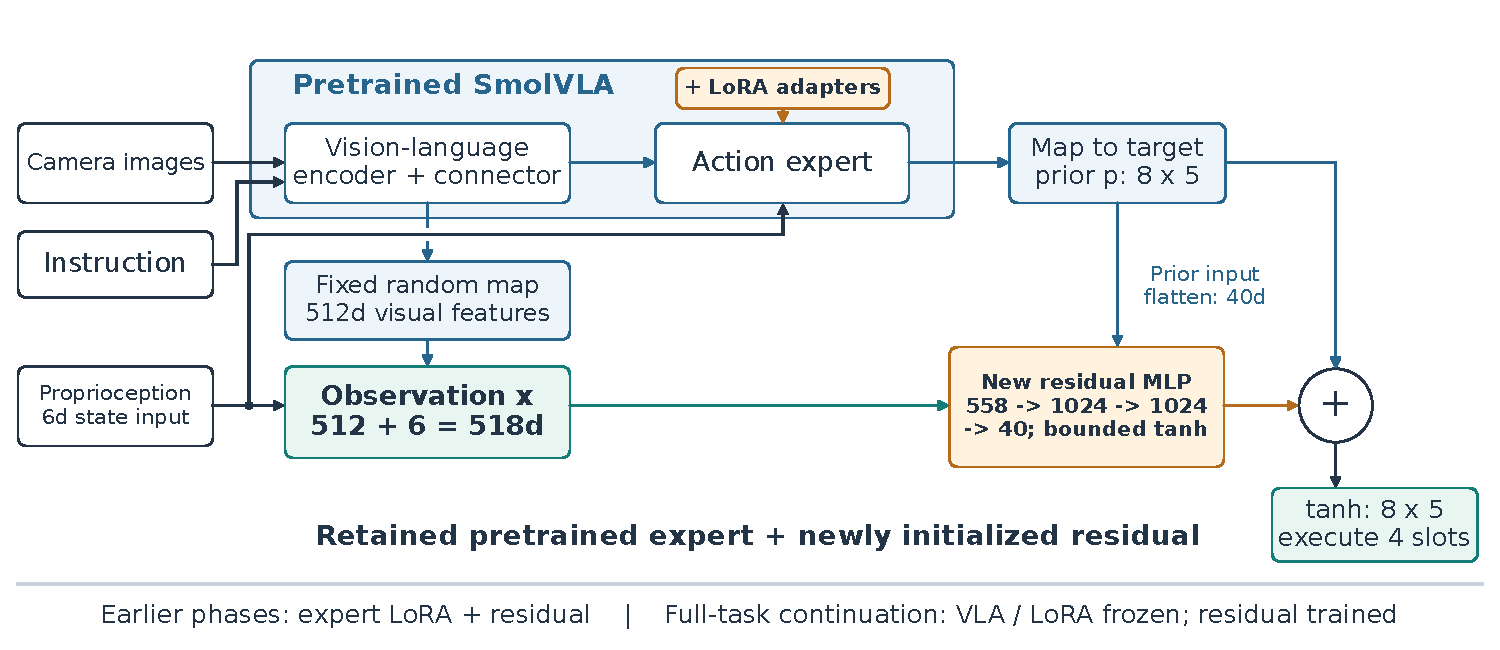
\includegraphics[width=\textwidth]{figures/smolvla_residual_lora.pdf}
\caption{SmolVLA implementation. The pretrained VLM and action expert are retained and frozen. A newly initialized residual combines 518 observation features with a 40-dimensional action prior. LoRA adapts the expert in supervised stages; the evaluated full-task continuation freezes the VLA and LoRA weights. Feature and action dimensions refer to the five-channel controller.}
\label{fig:architecture}
\end{figure*}

Figure~\ref{fig:architecture} and Table~\ref{tab:modules} describe the evaluated controller. The SmolVLA vision-language model and action expert are loaded from pretrained weights and are never reset or directly trained. Their action chunk is mapped to the five target channels; eight action slots form a 40-dimensional prior. Following the residual principle of PLD~\cite{pld}, a residual MLP is created with default initialization at the start of adaptation and is the component trained from scratch. It receives a 518-dimensional observation and the prior, and predicts a bounded correction; the combined action is bounded before execution. The observation consists of six proprioceptive values and a 512-dimensional visual feature. This feature is a fixed random projection of SmolVLA's connector tokens from both cameras. It is neither pretrained nor learned.

LoRA adapters on the action expert start with zero contribution. They are updated only in supervised stages, including the seeding stage, and are frozen during all full-task RL. During full-task training, only the residual and the exploration parameters change. The backbone, action mapping, and feature dimensions can change with the embodiment; the training schedule remains the same.

\begin{table}[!t]
\caption{Modules of the evaluated controller.}
\label{tab:modules}\centering\footnotesize
\setlength{\tabcolsep}{3pt}
\begin{tabular}{@{}lllr@{}}\toprule
Module & Initialization & Trained & Params\\\midrule
SmolVLA VLM & Pretrained & Never & $\approx$350M$^a$\\
SmolVLA action expert & Pretrained, not reset & Never & $\approx$100M$^a$\\
Expert LoRA (r\,=\,16, $\alpha$\,=\,32) & Zero update & SFT stages & 3.42M\\
Visual projection & Fixed random & Never & ---$^b$\\
Residual MLP & New (default) & All stages & 1.66M\\
Exploration $\log\sigma$ & Constant $-1.2$ & RL stages & 40\\\bottomrule
\end{tabular}\\[2pt]
\raggedright\footnotesize$^a$As documented for the 450M SmolVLA~\cite{smolvla}. $^b$Fixed $30{,}720\times512$ map.
\end{table}

\subsection{Milestone-Based Full-Task Composition}\label{sec:composition}
After skill consolidation, the base policy learns the complete task from empty-gripper starts using binary milestone rewards. The full-task prompt is \emph{put \textless object\textgreater\ into \textless destination\textgreater}, where the destination is plate or bowl. This includes the plate wording \emph{into plate}, whereas the isolated plate-placement skill uses \emph{on the plate}. The full-task instruction stays fixed throughout approach, pickup, and placement. Continuous dense shaping is confined to the initial simple-skill acquisition in Section~\ref{sec:skill_acquisition}. The LIBERO reward comparison examines how intermediate feedback can support execution of a complete instruction.

\label{sec:dense_method}
We consider terminal-only, phase-only, and combined dense-and-phase rewards. The combined reward uses a manually defined sequence of reach, grasp, lift, move, and place phases, with a hand-specified progress function for each phase.

At each simulator step, the tracker uses object and gripper state to compute progress for the active phase. Reaching progress increases as gripper--object distance decreases; grasping combines proximity with gripper closure and grasp state; lifting uses height gained above the initial object position; transport uses planar object--target distance; placement uses target proximity, release, and environment success. Each progress measure is normalized to the interval from zero to one. For progress $p_t$ and the phase's previous maximum $p_{\rm best}$, the rewarded increment is $\max(p_t-p_{\rm best},0)$. A completion predicate advances the tracker to the next phase and produces a phase bonus. The weighted progress increment and phase bonus are bounded and combined with terminal feedback. The native task-success verifier remains unchanged.

In the phase-only condition, the continuous progress weight is zero, leaving phase-completion bonuses and terminal feedback.

This construction needs a progress function, normalization, and state variables for every phase of each new task. Our adaptation pipeline therefore uses dense feedback only for simple skills, and full-task training uses binary milestones defined by completion predicates.

The motivation follows from a simple group calculation. For $G$ independent rollouts from one scene, each with success probability $p$, the probability of observing both success and failure is
\begin{equation}
P_{\rm mixed}=1-p^G-(1-p)^G.
\label{eq:mixed}
\end{equation}
With eight rollouts, this probability is only 21.6\% at 3\% success, but 94.2\% at 30\% success. Milestones can therefore provide informative comparisons before complete-task success becomes common.


Three ordered, irreversible milestones are defined by predicates on the simulator state. Approach ($M_1$) requires entering a 3\,cm neighborhood of the grasp point with the gripper open and the object undisplaced. Pickup ($M_2$) requires a persistent physical grasp and a lift of at least 5\,cm while held. Placement ($M_3$) requires the strict destination contract: correct receptacle, intentional release, settled geometry, and no carry slip or wrong placement. Each milestone pays $+1$ once.

The rule is simple: a later placement failure should not remove local credit for a successful approach or pickup. Actions up to the one that triggers $M_1$ form the approach segment, actions up to $M_2$ form the pickup segment, and later actions form the placement segment. Each segment receives its own group-relative advantage, computed among the eight rollouts of the same scene. Groups without variation in a segment are dropped from that segment, and the three segment losses receive equal weight. Full-task completion adds a bonus of 1 to the return. A negative completion advantage is suppressed on segments whose milestone was achieved. The policy still executes the complete instruction without an external controller switching between specialists.

\subsection{Stabilized Updates and Full-Task Continuation}\label{sec:rl_loss}
We use a clipped group-relative policy loss with entropy regularization:
\begin{equation}
\mathcal L_{\rm RL}=\mathcal L_{\rm clip}-\eta\mathcal H.
\label{eq:rl_loss}
\end{equation}
$\mathcal L_{\rm clip}$ is the PPO surrogate on the likelihood ratio of each rollout's actions, with the group-normalized advantage of its segment. It uses separate lower and upper clipping bounds, 0.20 and 0.28. The entropy term $\mathcal H$, weighted by $\eta=2\times10^{-4}$, maintains exploration during manipulation and composition. Together, these choices keep early updates conservative while successful behavior is still rare.

During skill learning, DAPO-style dynamic sampling filters uninformative groups and collects additional rollout groups within the configured collection budget~\cite{dapo}. With binary rewards, uniform outcomes provide no group-relative contrast. During dense acquisition, filtering instead checks within-group return variation, so partial progress can provide a learning signal before a group contains a successful skill execution.

During full-task continuation, the inherited VLA and LoRA remain frozen while the residual and exploration scale are trained with a fresh optimizer and the same milestone rewards. The controller adds Gaussian exploration noise and an episode-level offset to its predicted mean before clipping the command for execution. The offset is sampled once per episode and applied during selected phases. We store the original sample and the applied offset, then use both to evaluate its likelihood under the old and new policies~\cite{capg}.

Let $\mu_{\theta,t}$ denote the controller's predicted mean, $\sigma_\theta$ the learned exploration scale, and $b_t$ the applied offset. The sampled command $u_t$ and executed action $a_t$ are
\begin{equation}
\begin{aligned}
u_t&\sim\mathcal N(\mu_{\theta,t}+b_t,\operatorname{diag}(\sigma_\theta^2)),\\
a_t&=\operatorname{clip}(u_t,-1,1).
\end{aligned}
\label{eq:latent_action}
\end{equation}
The likelihood ratio scores the stored $u_t$ conditional on the same $b_t$. Section~\ref{sec:cdpr_results} reports complete-task performance.
